\documentclass{llncs}

\usepackage{fancyhdr}
\usepackage{flushend}
\usepackage{amsfonts,amssymb,amsmath,alltt}
\usepackage{stmaryrd}
\usepackage{xspace}
\usepackage{graphicx}
\usepackage{color}

\usepackage{makeidx}
\pagestyle{plain}
\usepackage[utf8]{inputenc}
\usepackage{url}
\usepackage[english]{babel}


\renewcommand{\ttdefault}{cmtt}
%This version DOES NOT suppress line breaks
% newcommands etc
\newenvironment{ttbox}{\begin{alltt}\ttbraces\small\tt}%
                      {\end{alltt}}
%the new definition of \. suppresses line breaks
\def\ttbraces{\let\.=\nobreak\chardef\{=`\{\chardef\}=`\}\chardef\|=`\\}

\newcommand{\symb}[1]{\makebox{\it #1}} 
\newcommand\ie{i.e.\!\,, }
\newcommand\rel{Re${\cal{L}}$}
%\newcommand{\TODO}[1]{\textcolor{red}{\textbf{[TODO:#1]}}}
%\newcommand*{\TODOfn}[2][noteC]{\TODO[#1]{[\footnote{\TODO[#1]{#2}}]}}
%\newcommand*{\TODOref}[2][todoC]{\TODOfn[#1]{\textbf{BIB-REF}: #2}}
\newcommand\ttand{\mbox{{$\land$}}}
\newcommand\ttor{\mbox{{$\lor$}}}
\newcommand\ttcap{\mbox{{$\cap$}}}
\newcommand\ttcup{\mbox{{$\cup$}}}
\newcommand\ttfun{\mbox{{$\Rightarrow$}}}
\newcommand\ttmimp{\mbox{{$\Longrightarrow$}}}
\newcommand\ttimp{\mbox{{$\longrightarrow$}}}
\newcommand\ttequiv{\mbox{{$\equiv$}}}
\newcommand\ttexists{\mbox{{$\exists$}}}
\newcommand\ttforall{\mbox{{$\forall$}}}
\newcommand\ttneg{\mbox{{$\neg$}}}
\newcommand\ttneq{\mbox{{$\neq$}}}
\newcommand\ttin{\mbox{{$\in$}}}
\newcommand\ttnin{\mbox{{$\notin$}}}
\newcommand\ttImp{\mbox{{$\Longrightarrow$}}}
\newcommand\ttlam{\mbox{\( \lambda \)}}
\newcommand\tttimes{\mbox{\( \times \)}}
\newcommand\ttlbrack{\mbox{\(\llbracket\)}}
\newcommand\ttrbrack{\mbox{\( \rrbracket \)}}
\newcommand\noie{\textit{i.e.},\xspace}
\newcommand\eg{~\textit{e.g.},\xspace}
\newcommand\noeg{\textit{e.g.},\xspace}
\newcommand\ttatI{\mbox{\( @_G \)}}
\newcommand\ttto[1]{\mbox{{$\to^{#1}$}}}
\newcommand\ttleq{\mbox{{$\le$}}}
\newcommand\ttrelI{\mbox{{$\to_{i}$}}}
\newcommand\ttrelIstar{\mbox{{$\to^*$}}}
\newcommand\ttrel[1]{\mbox{{$\to_{#1}$}}}
\newcommand\ttrelstar[1]{\mbox{{$\to_{#1}^*$}}}
\newcommand\ttalpha{\mbox{{$\alpha$}}}
\newcommand\ttsupseteq{\mbox{{$\supseteq$}}}
\newcommand\ttupdownarrow{\mbox{{$\Updownarrow$}}}
\newcommand\ttbigcap{\mbox{{$\bigcap$}}}
\newcommand\tttau{\mbox{{$\tau$}}}
\newcommand\ttsubseteq{\mbox{{$\subseteq$}}}
\newcommand\ttf{\mbox{{$f$}}}
\newcommand\ttvdash{\mbox{{$\vdash$}}}
\newcommand\ttref[1]{\mbox{\(\sqsubseteq_{#1}\)}}
\newcommand\ttrefV{\mbox{{$\sqsubseteq_V$}}}
\newcommand{\ttcalN}[1]{\mbox{{${\mathcal{N}}_{\texttt{#1}}$}}} 
\newcommand\ttNatt{\mbox{{$\mathcal{N}$}}}
\newcommand\ttattand[1]{\mbox{{$\oplus_{\wedge}^{#1}$}}}
\newcommand\ttattor[1]{\mbox{{$\oplus_{\vee}^{#1}$}}}
\newcommand\ttsigma{\mbox{{$\sigma$}}}
\newcommand\ttmref[1]{\mbox{{$\sqsubseteq_{#1}$}}}
\newcommand\ttmeref{\ttmref{\mathcal{E}}}
\newcommand\ttsn{\mbox{{\texttt{s}$_0$}}}
\newcommand\ttsigmap{\mbox{{$\sigma'$}}}
\newcommand\ttecal{\mbox{$\mathcal{E}$}}
%\newcommand\ttimg{\mbox{$\triangleleft$}}
\newcommand\ttimg{\mbox{\texttt{`}}}

\begin{document}
\frontmatter
  
\mainmatter
\title{Modeling and analyzing the Corona-virus warning app with the Isabelle Infrastructure framework}
\author{Florian Kamm\"uller and Bianca Lutz}

\institute{Middlesex University London and\\ Technische Universit\"at Berlin\\
\email{f.kammueller@mdx.ac.uk|bialut@gmail.com}
}
\maketitle
\begin{abstract}
We provide a model in the Isabelle Infrastructure framework of the recently published German
Corona-virus warning app. The app supports breaking infection chains by informing users
whether they have been in close contact to an infected person. The app has a decentralized
architecture that supports anonymity of users.
We provide a formal model of the existing app with the Isabelle Infrastructure framework
to show up some natural attacks in a very abstract model. We then use the security
refinement process of the Isabelle Infrastructure framework to highlight how the use of
continuously changing ephemeral ids improves the anonymity.
\end{abstract}

\section{Introduction}
\label{sec:intro}
The German Chancellor Angela Merkel has strongly supported the publication of
the mobile phone Corona-virus warning app (CWA; \cite{cwa:github}) by publicly proclaiming that the ``Corona
App deserves your trust'' \cite{bundes:20}. Many millions of mobile phone users
in Germany have downloaded the app with 6 million on the first day.
CWA is one amongst many similar applications that aim at the very important goal
to ``break infection chains'' by providing timely information to users of whether they
have been in close proximity to a person who tested positive for COVID-19.

%The CWA
%has taken a long time to develop being published only on
%16th June 2020. It
%was a quite costly project but this was mainly due to the management of
%Telekom and SAP being in the driving seat. But the app has been designed with great
The app was designed with great
attention on privacy: a distributed architecture \cite{cwa:arch} has been adopted %after a long and
%heated debate with supporters of a central architecture. The distributed architecture is
that is
based on a very clever application design whereby clients broadcast
highly anonymized so called ``Ephemeral IDs'' via Bluetooth and
store those ids of people in close proximity.
%highly anonymized so called ``Ephemeral IDs'' at physical locations via the
%Bluetooth Low Energy Beacon protocol.
%The app saves those ids of people in close proximity.
Infected persons report their infection by uploading their ids to a central server, providing all clients the means to assess exposure risk locally,
hence, stored contact data has never to be shared.
%Infected persons report their infection to a central server,
%which, in turn, provides all clients the means to reconstruct the ids
%used by reported cases over the last 14 days.
%
%When at a later date an infected person reports his infection to a central server,
%all clients are provided the means to reconstruct the ids used by this particular
%person's device over the last 14 days.
%Therefore, exposure risks can be evaluated locally and stored contact data has never to be shared.
%
%, the unique root ID is published
%and in the daily check all mobile phones connecting to the central server download
%the root IDs of infected people. Since the Ephemeral IDs can be mapped to the root ID
%all Ephemeral IDs that have been saved over the last 14 days allow users' phones to
%regularly check whether their user has been exposed to an infected person and issue
%a warning to the user and recommendation to contact health authorities.
%The warning issued by the Corona warning app entitles to
%having a Corona test done (which at the time of writing is not normally possible).

The Isabelle Infrastructure framework \cite{kam:20a} allows modeling and analyzing
architecture and scenarios including physical and logical entities, actors, and policies
within the interactive theorem prover Isabelle supported with temporal logic, Kripke
structures, and attack trees. It has been applied for example to Insider analysis in
airplanes \cite{kam:20b}, privacy in IoT healthcare \cite{kam:18b}, and recently also
to blockchain protocols \cite{kn:20}.

%{Motivation: Why bother re-engineering a formal specification for a nicely developed privacy oriented app? physical aspects (adoption rate), formal proof etc}
The technical advantage of modeling an application in the Isabelle Insider framework lies
in (a) having explicit representations of infrastructures, actors and policies in a
formal model that (b) allows additional automated verification of security properties
with CTL, Kripke structures and Attack Trees within the interactive theorem prover
Isabelle.

The app now in use in Germany has been developed based on a protocol proposed by the DP-3T project \cite{dp3t:github}:
A sophisticated security concept
conceived by experts in the field that has strong claims with regard to mathematical support \cite{dp3t:wp} [p2].
%The Corona-virus app has been produced based on a sophisticated security
%concept conceived by experts in the field %to our knowledge, no formal verification
%%
%and has strong claims with regard to mathematical support:
%
%``Such a design builds on strong, mathematically provable support for privacy and data protection goals [...]'' \TODOref{DP-3T Whitepaper p. 2} \smallskip\\
%  \NOTE{DP-3T on their design and how wisely chosen it is ;) We have to use this! Something along the l%ines of:}
%
However, there has, as of yet, to our knowledge no formal verification been involved.
Even if a ``post-production'' formal specification seems pointless, 
it allows to reveal weak points of the architecture, show that the measures that have
been conceived are suitable to cover those weak points,
or to what extent trade offs have to be made due to inherent vulnerabilities.
The protocol implemented by the framework CWA resembles only the most basic
of the three protocols proposed by the DP-3T project.
Hence, a formal verified model that stresses the impact or limits of certain security measures
might give more weight to appeals like \cite{dp3t:impl}
%to Apple and Google
to adopt the more sophisticated protocols.
%
%Thereby, we believe
%that our current work is useful to increase the trust in the Corona-virus app necessary for
%its wide adoption which in turn is crucial for it to be efficient.

The contributions of this paper are (a) formal re-engineering of the Corona-virus warning app
(b) providing an additional security and privacy analysis with interactive theorem proving
certification of a novel view on the system architecture including actors, locations, and policies,
(c) a formal definition of a security refinement process that allows to improve a system
based on attacks found by the attack tree analysis and (d) an application of the refinement to
improve security of the Corona-virus app specification.

In this paper, we first provide some background in Section \ref{sec:background}:
we give a brief overview of related works
and the protocol of the German app (Section \ref{sec:history}).
We then introduce the Isabelle Infrastructure framework (Section \ref{sec:isainf}).
Next, we present our model (Section \ref{sec:model}) and analysis of privacy and
attacks (Section \ref{sec:ana}). The found attack on the first abstract specification
motivates refinement. The formal definition of refinement for the Isabelle Infrastructure
framework is introduced and illustrated on the Corona-virus warning app (Section \ref{sec:ref})
before drawing some conclusions (Section \ref{sec:concl}).

The formal model in the Isabelle insider framework is fully mechanized and proved in
Isabelle (sources available \cite{kam:18smc}). 

\section{Background and related work}
\label{sec:background}
\subsection{DP-3T and PEPP-PT}
\label{sec:history}
We are mainly concerned with the architecture and protocols proposed by the
DP-3T (\textit{Decentralized Privacy-Preserving Proximity Tracing}) project \cite{dp3t:github}.
The main reason to focus on this particular family of protocols is the
\textit{Exposure Notification Framework} (ENF), jointly published by Apple and Google \cite{enf:proj}, that adopts
%the main
core principles of the DP-3T proposal. This API is not only used in the German
Corona-virus warning app but has the potential of being widely adopted in future
app developments that might emerge due to the reach of players like Apple and Google.

There are, however, competing architectures noteworthy, namely protocols developed under the
roof of the \textit{Pan-European Privacy-Preserving Proximity Tracing} project (PEPP-PT) \cite{pepppt:github}, e.g.
PEPP-PT-ROBERT \cite{pepppt:ROBERT},
that might be characterized as centralized architectures.

Neither DP-3T nor PEPP-PT are synonymous for just one single protocol. Each project endorses
different protocols with unique properties in terms of privacy and data protection.
%Yet, on a higher level of abstraction, it seems feasible to distinguish two basic architectures:
%protocols as endorsed by PEPP-PT might be characterized as centralized architectures whereas
%DP-3T-inspired protocols follow a (more) decentralized approach.\footnote{%
%  DP-3T involves a central backend server. It is decentralized with regard to
%  the collection and evaluation of contact information:
%  In centralized architectures the server provides a risk scoring services, whereas decentralized
%  approaches rely on local risk assessment and, thus, do not need to share contact information with
%  the backend.}

There is a variety of noteworthy privacy and security issues. %that deserve formal consideration (and verification).
The debate among %emerging between
advocates of centralized architectures and those in favor of a decentralized approach in particular yields a lot of interesting material detailing different attacks and possible mitigation strategies: \cite{pepppt:dp3tana}, \cite{pepppt:dp3tresp}, \cite{dp3t:psre}.

In terms of attack scenarios, we focus on, what might be classified as deanonymisation attacks: Tracking a device (see \cite{dp3t:psre}[p9], \cite{pepppt:dp3tana}[p8]) and identifying infected individuals (\cite{dp3t:psre}[p5], \cite{pepppt:dp3tana}[p9]).
%As first step, both attacks start with deanonymizing Ephemeral Ids,
%i.\,e. linking them the particular devices.
%Both attacks rely on deanonymisation of Ephemeral Ids,
%i.\,e. linking ids to particular devices.

\subsubsection{Basic DP-3T architecture}
%All DP-3T protocols roughly work the same:
%\subsubsection{Basic DP-3T protocol: How does it work?}
%  How does it relate to ENF/CWA? (broad strokes)}
%
Upon installation, the app generates secret daily seeds to derive \textit{Ephemeral Ids}
(EphIDs) from them. EphIDs are generated locally with cryptographic methods and cannot be connected
to one another but only reconstructed from the secret seed they were derived from.

During normal operation each client broadcasts its EphIDs via Bluetooth whilst scanning for
EphIDs broadcasted by other devices in the vicinity. Collected EphIDs are stored locally along
with associated meta-data such as signal attenuation and date. In DP-3T the contact information
gathered is never shared but only evaluated locally.

If patients test positive for the Corona-virus, they are entitled to upload specific data to a
central backend server. This data is aggregated by the backend server and redistributed to all
clients regularly to provide the means for local risk scoring, i.\,e., determining whether collected
EphIDs match those broadcasted by now-confirmed Corona-virus patients during the last, e.\,g., 14, 
days.

In the most simple (and insecure) protocol proposed by DP-3T %\cite{dp3t:wp}[p14ff]
this basically translates into publishing the daily seeds used to derive EphIDs from.
The protocol implemented by ENF and,
hence, CWA adopts this low-cost design \cite{cwa:arch}. DP-3T proposes two other, more sophisticated protocols that improve
privacy and data protection properties to different degrees but are more costly to implement.
%Aside from additional security measures,
%\TODOfn[styC]{In short: I want to name it but don't talk about it (since we're not really concerned with% this level of detail). But this sounds just sh...}
%like signing content the server provides as a general rule, the protocol implemented by ENF and,
%hence, CWA follows this low-cost design.\TODOref{CWA solution architecture ($\rightarrow$ github:CWA); probably ENF specification} DP-3T proposes two other, more sophisticated protocols that improve
%privacy and data protection properties to different degrees but are more costly.
%%TODOfn[styC]{``complicated'' sounds lame but ``costly'' is, perhaps, to simple/literal} to set up.
%\pagebreak

Figure \ref{fig:dp3tprot} illustrates the basic system architecture
along with some of the mitigation measures either implemented in CWA or proposed by DP-3T.
\begin{figure}[htb]
\vspace{-.5cm}
  \begin{center}
    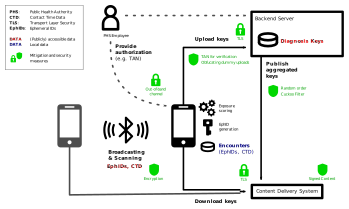
\includegraphics[width=4in]{DP-3T_basic_protocol}
  \end{center}
\vspace{-.5cm}
  \caption{Decentralized privacy-preserving proximity tracing protocol of CWA}
  \label{fig:dp3tprot}
\vspace{-.5cm}
\end{figure}

%\subsubsection{Attack scenarios}
%There is a variety of noteworthy privacy and security issues. %that deserve formal consideration (and verification).
%The debate among %emerging between
%advocates of centralized architectures and those in favor of a decentralized approach in particular yields a lot of interesting material detailing different attacks and possible mitigation strategies: \cite{pepppt:dp3tana}, \cite{pepppt:dp3tresp}, \cite{dp3t:psre}.

%In terms of attack scenarios, we focus on, what might be classified as deanonymisation attacks: Tracking a device (see \cite{dp3t:psre}[p9], \cite{pepppt:dp3tana}[p8]) and identifying infected individuals (\cite{dp3t:psre}[p5], \cite{pepppt:dp3tana}[p9]).
%%As first step, both attacks start with deanonymizing Ephemeral Ids,
%%i.\,e. linking them the particular devices.
%Both attacks rely on deanonymisation of Ephemeral Ids,
%i.\,e. linking ids to particular devices.

\subsection{Isabelle Infrastructure framework}
\label{sec:isainf}
%\TODO{Adapt: this is copied from FMBC paper}
The Isabelle Infrastructure is built in the interactive generic theorem prover
Isabelle/HOL \cite{npw:02}. As a framework, it supports formalization and proof of
systems with actors and policies. It originally emerged from verification of insider 
threat scenarios but it soon became clear that the theoretical concepts, like temporal
logic combined with Kripke structures and a generic notion of state transitions were
very suitable to be combined with attack trees into a formal security engineering process
\cite{suc:16} and framework \cite{kam:19a}.
%\subsubsection{Overview}
%\label{sec:isainfover}
Figure \ref{fig:theorystruc} gives an overview of the Isabelle Infrastructure 
framework with its layers of object-logics -- each level below embeds the one
above showing the novel contribution of this paper in blue on the top. 
\begin{figure}
\vspace{-.5cm}
  \begin{center}
  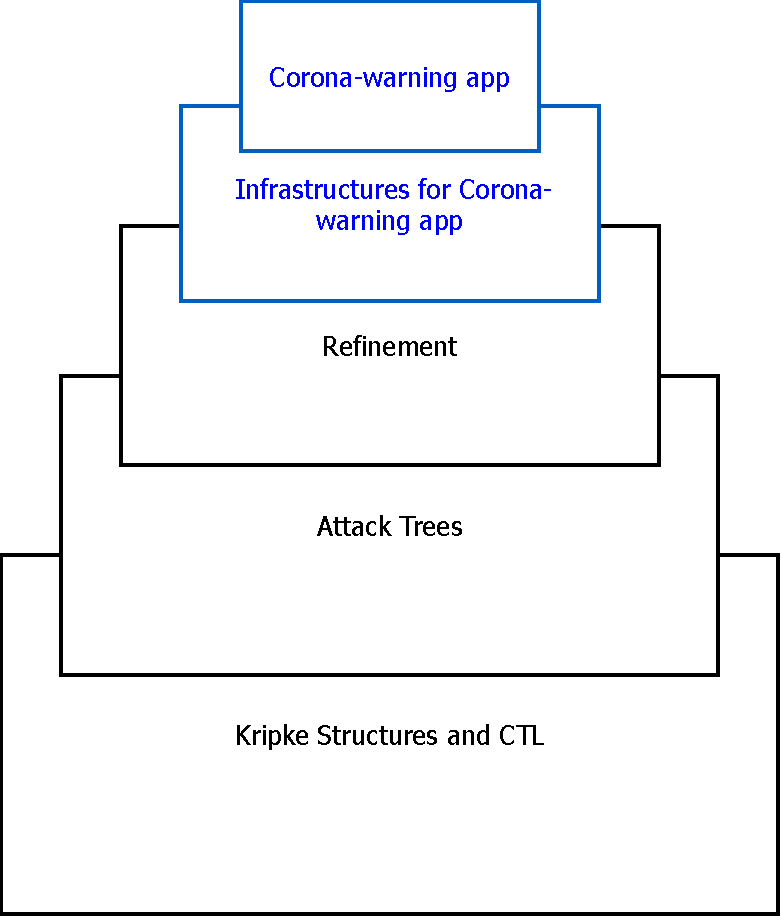
\includegraphics[scale=.35]{theory_structure.pdf}
\end{center}
\vspace{-.5cm}
\caption{Generic Isabelle Infrastructure framework applied to Corona-warning app.}
\label{fig:theorystruc}
\vspace{-.5cm}
\end{figure}


\subsubsection{Kripke structures, CTL, and Attack Trees}
\label{sec:intro}
The Isabelle framework has now after various case studies become a general framework for
the state-based security analysis of infrastructures with policies and actors. Temporal logic
and Kripke structures build the foundation. 
Meta-theoretical results have been established to show equivalence between attack trees 
and CTL statements \cite{kam:18b}. 
%As part of the meta-theory Correctness and Completeness have been 
%proved in Isabelle \cite{kam:18b} and can be used to navigate between CTL and attack 
%trees to find attacks. 
This foundation provides a generic notion of state transition on which attack trees and
temporal logic can be used to express properties. 
The main notions used in this paper are:
\begin{itemize}
\item {Kripke structures and state transitions:}\\ 
Using a generic state transition relation $\mapsto$, Kripke structures
are defined as a set of states reachable by $\mapsto$ from an initial
state set, for example
\begin{ttbox}
Kripke \{t. \ttexists i \ttin I. i \ttrelIstar t\} I
\end{ttbox}
\item {CTL statements:}\\ 
For example, we can write 
\begin{ttbox}
K \ttvdash {\sf EF} s
\end{ttbox}
to express that in Kripke structure \texttt{K} there is a path on which
the property \texttt{s} (a set of states) will eventually hold.
\item {Attack trees:} \\
The datatype of attack trees has three constructors: 
$\oplus_\vee$ creates or-trees and $\oplus_\wedge$ creates 
and-trees.
And-attack trees $l \ttattand s$ and or-attack trees $l \ttattor s$ 
consist of a list of sub-attacks -- again attack trees. The third constructor 
creates a base attack as a pair of state sets written \texttt{\ttcalN{(I,s)}}.
For example, a two step and-attack leading from state set \texttt{I} via
\texttt{si} to \texttt{s} is expressed as
\begin{ttbox}
\ttvdash [\ttcalN{(I,si)},\ttcalN{(si,s)}]\ttattand{\texttt{(I,s)}}
\end{ttbox}
%\begin{ttbox}
%\ttvdash [\ttcalN{(I,s)},\ttcalN{(s,s')}]\ttattand{(I,s')}
%\end{ttbox}
\item {Attack tree refinement, validity and adequacy:}\\
Attack trees have their own refinement (not to be mixed up with the
system refinement presented in this paper as introduced in the next section).
An abstract attack tree may be refined by spelling out the attack steps until a valid attack
is reached:

\texttt{\ttvdash A :: (\ttsigma :: state) attree)}.

The validity is defined constructively (code is generated from it)
and its adequacy with respect to a formal semantics in CTL is proved
and can be used to facilitate actual application verification as demonstrated 
her in the stepwise system refinements.
\end{itemize}


\subsubsection{Instantiation of Framework}
The formal model of the Corona-warning app uses the Isabelle Infrastructure framework instantiating it
by reusing its concept of {\it actors} for users and smartphones whereby locations correspond
to physical locations. The Ephemeral Ids, their sending and change is added to Infrastructures
by slightly adapting the basic state type of infrastructure graphs and accordingly the semantic rules
for the actions move, get, and put. The details of the newly adapted Infrastructure are
presented in Section \ref{sec:model}.
Technically, an Isabelle theory file \texttt{Infrastructure.thy} builds on top of the theories for Kripke 
structures and CTL (\texttt{MC.thy}), attack trees (\texttt{AT.thy}), and security refinement 
(\texttt{Refinement.thy}). Thus all these concepts can be used to specify the formal model
for the Corona-virus warning app, express relevant and interesting properties, and conduct
interactive proofs (with the full support of the powerful and highly automated proof support
of Isabelle).
%The Corona-virus warning app theory itself is an adaptation of the Infrastructure theory of the 
%Isabelle Infrastructure framework and reuses (or slightly adapts) existing concepts. 
%In the remainder of this paper, we introduce the model that we conceived for . 
All Isabelle sources are available online \cite{kam:20gitsc}.

\subsubsection{Refinement}
An additional feature that has been integrated into the Isabelle Infrastructure
framework motivated by security engineering formal specifications for IoT healthcare
system is an extension of the formal specification process introducing
refinement of Kripke structures \cite{kam:19a,kam:20a}. It refines a system model based on a 
formal definition of a combination of trace refinement and structural 
refinement (or datatype refinement). The definition allows to prove property preservation results 
crucial for an iterative development process.
The refinements of the system specification  can be interleaved with attack 
analysis while security properties can be proved in Isabelle. In each iteration
security qualities are accumulated while continuously attack trees scrutinize
the design.
One of the contributions of this paper is to explore different concepts of refinement:
the formal expression of refinement, enables to pin down (i.e. exemplify) different concepts
of refinement (data refinement, action refinement, trace refinement (aka spec refinement) and
combinations thereof with concrete attack scenarios. 

\section{Modeling and analyzing Corona-warning app}
\label{sec:model}
\subsection{Infrastructures, Policies, and Actors}
\label{sec:infra}
% Adapted from CSF paper
The Isabelle Infrastructure framework supports the representation of infrastructures 
as graphs with actors and policies attached to nodes. These infrastructures 
are the {\it states} of the Kripke structure. % for the attack trees.

The transition between states is triggered by non-parameterized
actions \texttt{get}, \texttt{move}, and \texttt{put} 
executed by actors. 
Actors are given by an abstract type \texttt{actor} and a function 
\texttt{Actor} that creates elements of that type from identities 
(of type \texttt{string} written \texttt{''s''} in Isabelle). 
Actors are contained in an infrastructure graph type \texttt{igraph}
constructed by its constructor \texttt{Lgraph}. 
\begin{ttbox}
{\bf datatype} igraph = 
         Lgraph (location \tttimes location)set 
                 location \ttfun identity set
                 identity \ttfun (string set \tttimes string set \tttimes efid)  
                 location \ttfun string \tttimes (dlm \tttimes data) set
                 location \ttfun efid set
                 actor \ttfun location \ttfun (identity \tttimes efid) set
\end{ttbox}
In the current application of the framework to the Corona-warning app case study, 
this graph contains a set of location pairs representing the %structure 
topology of the infrastructure
as a graph of nodes and a function%\footnote{ We use the common $\lambda$-abstraction, 
%e.g. \texttt{\ttlam x. True}, to define functions with parameters, here the 
%function returning True for any input $x$.} 
that assigns a set of actor identities to each node (location) in the graph.
The third component of an \texttt{igraph} assigns the credentials to each actor: 
a triple-valued function whose first range component is a set describing the credentials 
in the possession of an actor and the second component 
is a set defining the roles the actor can take on; 
most prominently the third component is the \texttt{efid} assigned to the actor. This is initially
just a natural number but will be refined to actually represent lists of ``Ephemeral'' Ids later
when refining the specification.
\begin{ttbox}
{\bf datatype} efid = Efid nat
\end{ttbox}
The fourth component of the type \texttt{igraph}
assigns security labeled data to locations, a feature not used in the
current application.
The second to last component assigns the set of efids of all currently present smart phones
to each location of the graph. The last component finally denotes the knowledge set of each
actor for each location: a set of pairs of actors and potential ids.

Corresponding projection functions for each of the components of an 
infrastructure graph are provided; they are named \texttt{gra} for the actual 
set of pairs of locations, \texttt{agra} for the actor map, \texttt{cgra} for 
the credentials, \texttt{lgra} for the %state of a location and the 
data at that location, \texttt{egra} for the assignment of current efids to locations,
and \texttt{kgra} for the knowledge set for each actor for each location.

In the Corona-virus warning app, the initial values for the \texttt{igraph} components use
two locations \texttt{pub} and \texttt{shop} to define the following constants (we omit the
data map component \texttt{ex\_locs}).
\begin{ttbox}
ex_loc_ass \ttequiv (\ttlam x. if x = pub then \{''Alice'', ''Bob'', ''Eve''\}  
                 else (if x = shop then \{''Charly'', ''David''\} 
                 else \{\}))
ex_creds \ttequiv (\ttlam x. if x = ''Alice'' then (\{\}, \{\}, Efid 1) else 
              (if x = ''Bob'' then  (\{\},\{\}, Efid 2) else 
              (if x = ''Charly'' then (\{\},\{\}, Efid 3) else
              (if x = ''David'' then (\{\},\{\}, Efid 4) else
              (if x = ''Eve'' then (\{\},\{\}, Efid 5)
               else (\{\},\{\},Efid 0))))))
ex_efids \ttequiv (\ttlam x. if x = pub then \{Efid 1, Efid 2, Efid 5\}
                  else (if x = shop then \{Efid 3, Efid 4\} else \{\}))
ex_knos \ttequiv (\ttlam x. (if x = Actor ''Eve'' then (\ttlam l. \{\} else (\ttlam l. \{\})))
\end{ttbox}  
These components are wrapped up into the following \texttt{igraph}.
\begin{ttbox}
ex_graph \ttequiv
      Lgraph \{(pub, shop)\} ex_loc_ass ex_creds ex_locs ex_efids ex_knos
\end{ttbox}  
Infrastructures are given by the following datatype that 
contains an infrastructure graph of type \texttt{igraph} 
and a policy given by a function that assigns local policies over a graph to
all locations of the graph. 
\begin{ttbox}
{\bf{datatype}} infrastructure = Infrastructure igraph 
                                         [igraph, location] \ttfun policy set
\end{ttbox}
There are projection functions \texttt{graphI} and \texttt{delta} when applied
to an infrastructure return the graph and the local policies, respectively.
The function \texttt{local\_policies} gives the policy for each location \texttt{x}
over an infrastructure graph \texttt{G} as a pair: the first element of this pair is 
a function specifying the actors \texttt{y} that are entitled to perform the actions 
specified in the set which is the second element of that pair.
The local policies definition for the Corona-warning app, simply permits all actions to
all actors in both locations.
\begin{ttbox}
  local_policies G \ttequiv
         (\ttlam x. if x = pub then  \{(\ttlam y. True, \{get,move,put\})\}
          else (if x = shop then \{(\ttlam y. True, \{get,move,put\})\} else \{\}))
\end{ttbox}  
For the Corona-warning app, the initial infrastructure contains the graph \texttt{ex\_graph}
with its two locations pub and shop and is then wrapped up with the local policies
into the infrastructure \texttt{Corona\_scenario} 
that represents the ``initial'' state for the Kripke structure.
\begin{ttbox}
 Corona_scenario \ttequiv Infrastructure  ex_graph local_policies
\end{ttbox}

\subsection{Policies, privacy, and behaviour}
\label{sec:}
Policies specify the expected behaviour of actors of an infrastructure. 
They are given by pairs of predicates (conditions) and sets of (enabled) actions.
%\begin{ttbox}
%{\bf type}_{\bf{synonym}} policy = ((actor \ttfun bool) \tttimes action set)
%\end{ttbox}
%The behaviour of actors is 
They are defined by the \texttt{enables} predicate:
an actor \texttt{h} is enabled to perform an action \texttt{a} 
in infrastructure \texttt{I}, at location \texttt{l}
if there exists a pair \texttt{(p,e)} in the local policy of \texttt{l}
(\texttt{delta I l} projects to the local policy) such that the action 
\texttt{a} is a member of the action set \texttt{e} and the policy 
predicate \texttt{p} holds for actor \texttt{h}.
\begin{ttbox}
enables I l h a \ttequiv \ttexists (p,e) \ttin delta I l. a \ttin e \ttand p h
\end{ttbox} 

The Privacy protection goal is to avoid deanonymization. That is, an attacker should not be able to
disambiguate the set of pairs of real Ids and EphIds. This is abstractly expressed in the predicate
identifiable.
\begin{ttbox}
identifiable eid A \ttequiv is_singleton\{(Id,Eid). (Id, Eid) \ttin A \ttand Eid = eid\}
\end{ttbox}
The predicate identifiable is used to express as the global policy `Eve cannot deanonymize an Ephemeral
Id \texttt{eid} using the gathered knowledge':
%{\bf fixes} global_policy::[infrastructure, identity] \ttfun bool
%{\bf defines}  
\begin{ttbox}
  global_policy I eid \ttequiv
             \ttneg(identifiable eid 
                ((\ttbigcap (kgra(graphI I)(Actor ''Eve'')`(nodes(graphI I))))
                 - \{(x,y). x = ''Eve''\}))
\end{ttbox}

\subsection{Infrastructure state transition}
\label{sec:statetrans}
The state transition relation uses the syntactic infix notation 
\texttt{I \ttrelI\, I'}  to denote that infrastructures 
\texttt{I} and \texttt{I'} are in this relation.
%Rules for the put, get, move, process and delete actions exist.
To give an impression of this definition, we show first the rule defining the state transition for
the action get. Initially, this rule expresses that
an actor that resides at a location \texttt{l} (\texttt{a \ttatI\ l})
and is enabled by the local policy in this location to ``get'' can
combine  all ids at the current location (contained in \texttt{egra G l}) with
all actors at the current location (contained in \texttt{agra G l}) and add this
set of pairs to his knowledge set \texttt{kgra G} using the function update \texttt{f(l := n)}
redefining the function \texttt{f} for the input \texttt{l} to have now the new value \texttt{n}.
\begin{ttbox}
 {\bf{get\_data}}: G = graphI I \ttImp a \ttatI l \ttImp enables I l (Actor a) get \ttImp 
   I' = Infrastructure 
          (Lgraph (gra G)(agra G)(cgra G)(lgra G)(egra G)
            ((kgra G)((Actor a) := ((kgra G (Actor a))(l:=
                 \{(x,y). x \ttin agra G l \ttand y \ttin egra G l\})))))
          (delta I)
   \ttImp I \ttrel{n} I' 
\end{ttbox}
Another interesting rule for the state transition is the one for \texttt{move} whose structure
resembles the previous one.
\begin{ttbox}
 {\bf{move}}: G = graphI I \ttImp a \ttatI l \ttImp a \ttin actors_graph(graphI I) \ttImp
    l \ttin nodes G \ttImp l' \ttin nodes G \ttImp enables I l' (Actor h) move \ttImp
    I' = Infrastructure (move_graph_a a l l' (graphI I))(delta I)
 \ttImp I \ttrelI I' 
\end{ttbox}
The semantics of this rule is embedded in the function \texttt{move\_graph\_a}
that adapts the infrastructure state so that the moving actor \texttt{a} is now
associated to the target location \texttt{l'} in the actor map \texttt{agra} and not
any more at \texttt{l} and also the association of \texttt{efids} is updated accordingly.
\begin{ttbox}
move_graph_a n l l' g \ttequiv
  Lgraph (gra g) 
         (if n \ttin ((agra g) l) \ttand  n \ttnin ((agra g) l') then 
           ((agra g)(l := (agra g l) - \{n\}))(l' := (insert n (agra g l')))
          else (agra g))
         (cgra g)(lgra g)
         (if n \ttin ((agra g) l) \ttand  n \ttnin ((agra g) l') then
               ((egra g)(l := (egra g l) - \{efemid (cgra g n)\}))
                        (l' := (insert (efemid (cgra g n))(egra g l')))
          else egra g)
         (kgra g)
\end{ttbox}  
Based on this state transition and the above defined \texttt{Corona\_scenario}, we define the first Kripke structure.
\begin{ttbox}
 corona_Kripke \ttequiv Kripke \{ I. Corona_scenario \ttrelIstar I \} \{Corona_scenario\}
\end{ttbox}

\subsection{Attack analysis}
\label{sec:ana}
For the analysis of attacks, we negate the security property that we want to achieve,
usually the global policy.

Since we consider a predicate transformer semantics, we use
sets of states to represent properties. 
%For example, the attack property
The invalidated global policy is given by the set \texttt{scorona}.
\begin{ttbox}
 scorona \ttequiv \{x. \ttexists n. \ttneg global_policy x (Efid n)\}
\end{ttbox}
The attack we are interested in is to see whether for the scenario
\begin{ttbox}
 Kripke\_scenario \ttequiv  Infrastructure ex_graph local_policies 
\end{ttbox}
from the initial state \texttt{Icorona \ttequiv \{corona\_scenario\}},
the critical state \texttt{scorona} can be reached,
that is, is there a valid attack \texttt{(Icorona,scorona)}?

For the Kripke structure \texttt{corona\_Kripke}
we first derive a valid and-attack using the attack tree proof calculus.
\begin{ttbox}
  \ttvdash [\ttcalN{(Icorona,Corona)},\ttcalN{(Corona,Corona1)},\ttcalN{(Corona1,Corona2)},
             \ttcalN{(Corona2,Corona3)},\ttcalN{(Corona3,scorona)}]\ttattand{\texttt{(Icorona,scorona)}}
\end{ttbox}
The sets \texttt{Corona, Corona1, Corona2, Corona3} are the intermediate states where
\texttt{Bob} moves to shop and \texttt{Eve} follows him collecting the Ephemeral Ids in each location.
The collected information enables identifying Bob's Ephemeral Id.

The attack tree calculus \cite{kam:18b} exhibits that an attack is possible.
\begin{ttbox}
 corona_Kripke \ttvdash {\sf EF} scorona
\end{ttbox}
We can simply apply the Correctness theorem \texttt{AT\_EF} to 
immediately prove this CTL statement. This application of the meta-theorem 
of Correctness of attack trees saves us proving the CTL formula tediously 
by exploring the state space in Isabelle proofs. Alternatively, we could use 
the generated code for the function \texttt{is\_attack\_tree} in Scala 
(see \cite{kam:18b}) to check that a refined attack of the above is valid.

\section{Refinement}
\label{sec:ref}
%\TODO{This section is just copied over from arxive paper - adapt}
Intuitively, a refinement changes some aspect of the type of
the state, for example, replaces a data type by a richer datatype or
restricts the behaviour of the actors. The former is expressed directly 
by a mapping of datatypes, the latter is incorporated into the state
transition relation of the Kripke structure that corresponds to the 
transformed model.
%This relationship between the Kripke structure can be better understood
%visually (see Figure \ref{fig:modtrans})
In other words, we can encode a refinement within our framework
as a relation on Kripke structures that is parameterized additionally by
a function that maps the refined type to the abstract type.
The direction ``from refined to abstract'' of this type mapping may seem 
curiously counter-intuitive. However, the actual refinement is given by the 
refinement that uses this function as an input. The refinement
then refines an abstract to a more concrete system specification. 
The additional layer for the refinement 
%(the red box in Figure \ref{fig:theorystruc})
can be formalized in Isabelle as a
%second\footnote{The first refinement 
%relation in this framework is on attack trees summarized in Section \ref{sec:at}.} 
refinement relation 
$\sqsubseteq_{\mathcal{E}}$. 
The relation \texttt{mod\_trans} is typed as a relation over triples --
a function from a threefold Cartesian product to \texttt{bool}, the 
type containing true and false only.  
The type variables $\sigma$ and $\sigma'$ input to the type constructor 
\texttt{Kripke} represent the abstract state type and the concrete state type. 
Consequently, the middle element of the triples selected by the relation 
\texttt{mod\_trans} is a function of type $\sigma' \Rightarrow \sigma$ 
mapping elements of the refined state to the abstract state.
The expression in quotation marks after the type is again the
infix syntax in Isabelle that allows the definition of mathematical notation
instead of writing \texttt{mod\_trans} in prefix manner. This nicer infix
syntax is already used in the actual definition.
Finally, the arrow \texttt{\ttImp} is the implication of Isabelle's  meta-logic
while $\ttimp$ is the one of the {\it object} logic HOL. 
They are logically equivalent but of different
types: within a HOL formula $P$, for example, as below $\forall x. P \ttimp Q$, only the implication $\ttimp$
can be used.
\begin{ttbox}
 refinement :: (\ttsigma Kripke \tttimes (\ttsigma' \ttfun \ttsigma) \tttimes \ttsigma' Kripke) \ttfun bool ("_ \ttmref{(\_)} _")
  K \ttmeref K' \ttequiv \ttforall s' \ttin states K'. \ttforall s \ttin init K'. 
             s \ttrelstar{\sigma'} s' \ttimp \ttecal(s) \ttin init K \ttand \ttecal(s) \ttrelstar{\sigma} \ttecal(s')
\end{ttbox}
The definition of \texttt{K \ttmeref\, K'} states that for any state $s'$ 
of the refined Kripke structure that can be reached by the state transition
in zero or more steps from an initial state $s$ of the refined Kripke 
structure, the mapping ${\mathcal E}$ from the refined to the abstract 
model's state must preserve this reachability, i.e., the image of
$s$ must also be an initial state and from there the image of $s'$
under ${\mathcal E}$ must be reached with $0$ or $n$ steps.

\subsection{Property Preserving System Refinement}
A first direct consequence of this definition is the following lemma
where the operator \texttt{$\ttimg$} in \texttt{\ttecal\ttimg(init K')}
represents function image, that is the set, $\{\ttecal(x). x \in \texttt{init K'}\} $.
\begin{ttbox}
{\bf{lemma}} init_ref: K \ttmeref K' \ttImp \ttecal\ttimg(init K') \ttsubseteq init K
\end{ttbox}
A more prominent consequence of the definition of refinement 
is that of property preservation. Here, we show that refinement preserves the
CTL property of ${\sf EF} s$ which means that a reachability property true in the
refined  model \texttt{K'} %has also been 
is already true in the abstract model.
A state set $s'$ represents a property %since we use 
in the predicate transformer view of properties as sets of states. 
The additional condition on initial states ensures that we cannot ``forget'' them. 
%initial states.
%The theorem states that, if the 
%property \texttt{{\sf EF} s'} is true in the concrete model its  has been true 
%can be reached from the initial state in 
%\texttt{K'} then it is also possible  to reach the image of this property
% in the abstract Kripke structure \texttt{K}.
\begin{ttbox}
{\bf{theorem}} prop_pres: 
   K \ttmeref K'  \ttImp init K \ttsubseteq \ttecal\ttimg(init K') \ttImp
   \ttforall s' \ttin Pow(states K'). K' \ttvdash {\sf EF} s' \ttimp K \ttvdash {\sf EF} (\ttecal\ttimg(s'))
\end{ttbox}
It is remarkable, that our definition of refinement by Kripke 
structure refinement entails property preservation and makes it possible 
to prove this as a theorem in Isabelle once for all, i.e., as a meta-theorem.
However, this is due to the fact that our generic definition of state transition
allows to explicitly formalize such sophisticated concepts like reachability.
For practical purposes, however, the proof obligation of showing that
a specific refinement is in fact a refinement is rather complex
justly because of the explicit use of the transitive closure of the state
transition relation.
In most cases, the refinement will be simpler. Therefore, we offer
additional help by the following theorem that uses a stronger characterization
of Kripke structure refinement and shows that our refinement follows
from this.
\begin{ttbox}
{\bf{theorem}} strong_mt: 
\ttecal\ttimg(init K') \ttsubseteq init K \ttand s \ttrel{\sigma'} s' \ttimp \ttecal(s) \ttrel{\sigma} \ttecal(s') 
\ttImp K \ttmeref K'
\end{ttbox}
This simpler characterization is in fact a stronger one: we could have $s \ttrel{\sigma'} s'$ 
in the refined Kripke structure \texttt{K'} and $\neg(\ttecal(s) \ttrel{\sigma} \ttecal(s'))$
but neither $s$ nor $s'$ are reachable from initial states in \texttt{K'}.
For cases, where we want to have the simpler one-step proviso but still need 
reachability we provide a slightly weaker version of \texttt{strong\_mt}.
\begin{ttbox}
{\bf{theorem}} strong_mt':  
\ttecal\ttimg(init K') \ttsubseteq init K \ttand (\ttexists s0 \ttin init K'. s0  \ttrelIstar s)
 \ttand s \ttrel{\sigma'} s' \ttimp \ttecal(s) \ttrel{\sigma} \ttecal(s') \ttImp K \ttmeref K'
\end{ttbox}
This idea of property preservation coincides with the classical idea of
trace refinement as it is given in process algebras like CSP. In this view,
the properties of a system are given by the set of its traces. Now, a refinement
of the system is given by another system that has a subset of the traces of the 
former one.
Although the principal idea is similar, we greatly extend it since our notion
additionally incorporates refinement. Since we include a state map 
\texttt{\ttsigma'\ttfun \ttsigma} in our refinement map, we additionally
allow structural refinement: the state map generalizes the basic idea of
trace refinement by traces corresponding to each other but allows additionally
an exchange of data types. 
As we see in the application to the case study, the refinement steps may
sometimes just specialize the traces: in this case the state map 
\texttt{\ttsigma'\ttfun \ttsigma} is just identity. 

In addition, we also have a simple implicit version of {\it action refinement}. In an
action refinement, traces may be refined by combining consecutive system events
into atomic events thereby reducing traces.
We can observe this kind of refinement in the second refinement step
%This will be detailed in the second refinement step
of the Corona-virus warning app considered next.

\subsection{Refining the Specification}
\label{sec:corref}
Clearly, fixed Ephemeral Ids are not really ephemeral. The model presented
in Section \ref{sec:model} has deliberately been designed abstractly to allow focusing on
the basic system architecture and finding an initial deanonymization attack.
We now introduce ``proper'' Ephemeral Ids and show how the system datatype can be refined to a system
that uses those instead of the fixed ones.

For the DP-3T Ephemeral Ids \cite{dp3t:wp}, for each day $t$ a seed $SK_t$
is used to generate a list of length $n = 24 * 60 / L$, where $L$ is the duration for which
the Ephemeral Ids are posted by the smart phone
\begin{ttbox}
  EphId1 || ... || EphIdn = PRG(PRF(SKt,``broadcast key''))
\end{ttbox} 
``where PRF is a pseudo-random function (e.g., HMAC-SHA256), ``broadcast key'' is a
fixed, public string, and PRG is a pseudorandom generator (e.g. AES in counter mode)'' \cite{dp3t:wp}.

From a cryptographic point of view, the crucial properties of the Ephemeral Ids are that
they are purely random, therefore, they cannot be guessed, but at the same time if -- after
the actual encounter between sender and receiver -- the seed $SK_t$ is published, it is feasible
to relate any of the \texttt{EphIDi} to $SK_t$  for all \texttt{i} $\in \{1, \ldots, n\}$.
For a formalization of this crucial cryptographic property in Isabelle it suffices to define a new type
of list of Ephemeral Ids \texttt{efidlist} containing the root $SK_t$ (the first \texttt{efid}),
a current \texttt{efid} indicated by a list pointer of type \texttt{nat}, and the actual list of
\texttt{efid}s.
\begin{ttbox}
{\bf{datatype}} efidlist = Efids "efid" "nat" "efid list"
\end{ttbox}
We define functions for this datatype: \texttt{efidsroot} returning the first of the three
constituents in an \texttt{efidlist} (the root $SK_t$); \texttt{efids\_index} giving the second
component, the index of the current \texttt{efid}; \texttt{efids\_inc\_ind} applied to an
\texttt{efidlist} increments the index; \texttt{efids\_cur} returning the current \texttt{efid}
from the list and \texttt{efids\_list} for the entire list (the third component).

The first step of refinement replaces the simple \texttt{efid} in the infrastructure type by the
new type \texttt{efidlist}. Note, that in the new datatype \texttt{igraph} this change affects only
the third component, the credentials to become
\begin{ttbox}
   identity \ttfun (string set \tttimes string set \tttimes efidlist)
\end{ttbox}
The last two components, the set of currently present efids,
and the knowledge set, remain the same and still operating on the simple type \texttt{efid}.
%\begin{ttbox}
%{\bf datatype} igraph =
%         Lgraph (location \tttimes location)set
%                 location \ttfun identity set
%
%                 location \ttfun string \tttimes (dlm \tttimes data) set
%                 location \ttfun efid set
%                 actor \ttfun location \ttfun (identity \tttimes efid) set
%\end{ttbox}
The refined state transition relation implements the possibility of changing the Ephemeral Ids
by the rule for the action \texttt{put} that resembles very much the rule for \texttt{get}.
%\begin{ttbox}
% {\bf{put}}: G = graphI I \ttImp  a \ttatI l \ttImp enables I l (Actor a) put \ttImp
%      I' = Infrastructure (put_graph_efid A l (graphI I))(delta I)
% \ttImp I \ttrelI I'
%\end{ttbox}
The important change to the infrastructure state is implemented in the function \texttt{put\_graph\_efid} that
increases the current index in the \texttt{efidlist} in the credential component \texttt{cgra g n} for
the ``putting'' actor identity \texttt{n} and inserts the current \texttt{efid} from that credential
component into the \texttt{egra} component, the set of currently ``present'' Ephemeral Ids at the location
\texttt{l}.
\begin{ttbox}
put_graph_efid n l g  \ttequiv
  Lgraph (gra g)(agra g)
         ((cgra g)(n := (credentials (cgra g n), roles (cgra g n),
                         efids_inc_ind(efemid (cgra g n)))))
         (lgra g)
         ((egra g)(l := insert (efids_cur(efemid (cgra g n)))(egra g l)))
         (kgra g)
\end{ttbox}
We can now apply the refinement by defining a datatype map from the refined infrastructure type
\texttt{InfrastructureOne.infrastructure} to the former one \texttt{Infrastructure.infrastructure}.
\begin{ttbox}
{\bf{definition}} refmap :: InfrastructureOne.infrastructure \ttfun
                          Infrastructure.infrastructure
{\bf{where}} refmap I =
  Infrastructure.Infrastructure 
    (Infrastructure.Lgraph
       (InfrastructureOne.gra (graphI I))
       (InfrastructureOne.agra (graphI I))
        (\ttlam h. repl_efr 
           (InfrastructureOne.cgra (graphI I)) h)
           (InfrastructureOne.lgra (graphI I))
           (InfrastructureOne.egra (graphI I))
           (\ttlam a. \ttlam l.
  (\ttlam (x,y).(x, efids_root(efemid(InfrastructureOne.cgra (graphI I) x))))
                       \ttimg(InfrastructureOne.kgra (graphI I)) a l))                                                    
\end{ttbox}  
This is then plugged into the parameter \texttt{\ttecal} of the refinement operator allowing to
prove \texttt{corona\_Kripke \ttref{\texttt{refmap}} corona\_KripkeO} where the latter is the
refined Kripke structure.

Surprisingly, we can still prove \texttt{corona\_KripkeO \ttvdash EF scoronaO} by using the
same attack tree as in the abstract model: if Bob moves from pub to shop, he is vulnerable to
being identifiable as long as he does not change the current \texttt{efid}. So, if Eve moves to
the shop as well and performs a get before Bob does a put, then Eve's knowledge sets permits identifying
Bob's current Ephemeral Id as his.

\subsubsection{Second refinement step}
The persistent attack can be abbreviated informally by the action sequence \texttt{[get,move,move,get]}
performed by actors Eve, Bob, Eve, and Eve again, respectively.
How can a second refinement step avoid that Eve does the last \texttt{get} by imposing that after the
first \texttt{move} of Bob a \texttt{put} action must happen before Eve can do another \texttt{get}?
A very simple remedy to exclude this attack is to bind a \texttt{put} action after every \texttt{move}.
We can implement that change by a minimal update to the function \texttt{move\_graph\_a} (see Section \ref{sec:model})
by adding an increment (highlighted in the code snippet)
of the currently used Ephemeral Id before updating the \texttt{egra} component of the target location.
\begin{ttbox}
move\_graph\_a n l l' g \ttequiv ...
  (l' := insert (efids_cur({\bf efids\_inc\_ind}(efemid (cgra g n))))(egra g l))...
\end{ttbox}  
This is an action refinement because the move action is changed. It is a refinement, since
any trace of the refined model can still be mapped to a trace in the more abstract model just
omitting a few steps (the refinement relation is defined using the reflexive transitive closure
\texttt{\ttrelIstar}.


\section{Summary and discussion of relevance of the approach}
%{Conclusions}
\label{sec:concl}
%\subsection{Protection goals of attacks}
%\subsection{Summary and discussion of relevance of the approach}
We can establish in our formal framework an attack that even a system using changing
Ephemeral ids can be broken if the attacker physically follows a victim. This is a basic attack on
anonymity: a user's connection between his Ephemeral Ids and personal details (Iphone MAC or name)
is revealed to the attacker. The protection goal of privacy is thereby destroyed.

When establishing the attack we start from a simplistic scenario that does not use Ephemeral Ids but fixed ids.
In this (over)simplified model the attack is established. We then define a formal Refinement calculus for
the Isabelle Infrastructure framework to refine the attack to a system with Ephemeral Ids that change in fixed
time intervals obfuscating the relationship between user and his pseudonym\footnote{We identify the smartphone
  and the user which might be also recognized by his appearance (face)}.

Now, the refinement shows that although the Ephemeral Ids change regularly the same attack that has been
identified on the very abstract level (fixed ids) persists.
The refinement allows refining the datatype (Id $\mapsto$ EphId) but also delivers the usual trace
refinement (behaviours of the refined systems are a subset of the traces of the abstract system).
This persistence of the attack precisely shows which part of the system behaviour is responsible for the
attack. In a second refinement step using action refinement based on this insight from the (repeated)
attack, we can exclude the dangerous attack trace.
%\footnote{Implication on the actual protection goals
%  that are endangered by the attack on privacy are discussed in the larger context of the Corona-warning
%  app (see previous Section)}.

Clearly, the abstract attack we establish is obvious on an informal level but the persistence of the attack
on the refined system is less obvious. The remedy by a second refinement step is an evident restriction of
the system behaviour which gives a clear specification of a system secured against this attack. The use of
formal methods therefore lies not in the discovery of an obvious attack on a simplified system but in showing
how a formal specification including security refinement can lead to a stepwise improvement that is accompanied
by formal proof in the Isabelle Infrastructure framework. The solution to exclude the attack in the second refinement
step binds the action move together with a put action. %which effectively represents an action refinement.
This shows that besides datatype refinement and trace refinement our Refinement calculus also entails action
refinement. This action refinement is implemented implicitly by changing the effects of the actions
in the semantic state transition relation. In future work, we could think about making the action refinement
more explicit by considering a relationship between semantic rules or by refining the refinement notion to
a more explicit layer of protocol steps -- similar to what has been done in previous applications of the
Isabelle Infrastructure framework for example to Auction protocols \cite{kkp:17} or the Quantum Key Distribution \cite{kam:19c}.

The security refinement in general might seem pointless, as in the first step of refinement the attack
persists and even though the second refinement gets rid of this specific attack, it doesn't exclude the
reachability of the attack goal altogether (if the attacker Eve gets Bob on his own in a location she can
map all used EphIDs to him).
However, the refinement makes the system relatively more secure in that for a larger number of traces the abstract
attack does not work anymore\footnote{Adding probabilities as in \cite{kam:19c} enables quantifying this.}. 
It is important to emphasize that security refinement is a cyclic process that
improves security but does not usually terminate (like a loop) with a fixed point of 100\% secure system.
In a refined model new detail may give rise to new attack possibilities. These additional attacks can be
identified using the Attack Tree calculus and trigger further refinement steps.

\bibliographystyle{abbrv}
\bibliography{insider}

\end{document}
